\chapter{Experimental Apparatus}
%\addcontentsline{toc}{chapter}{Experimental Apparatus}

\section{The Large Hadron Colider}
\subsection{Injector Chain}
\subsection{The LHC}
\subsection{Experiments}

\section{The ATLAS Detector}

The ATLAS detector (shown in figure \ref{fig:ATLAS_overview}) is a multi-purpose detector designed to make precision measurements of various Standard model phenomena, investigate the Higgs sector and to search for new physics signals. The detector itself is radiation hard (in particular the tracking systems) and highly granular in order to deal with high event rates and intense pile up conditions at the Large Hadron Collider (LHC). It has coverage to high values of pseudorapidity $\eta$ and full coverage in azimuthal angle $\phi$\footnote{The ATLAS detector used a right handed coordiante system with the following conventions. The $x$ axis points towards the centre of the LHC ring, the $y$ axis points vertically upwards and the $z$ axis poitns anti-clockwise along the beamline when viewed from above.}. The detector is constructed in layers with the tracking systems in the centre, followed by the calorimeters and finally the muon systems. Details of all major components are described below.

\begin{figure}
  \begin{center}
    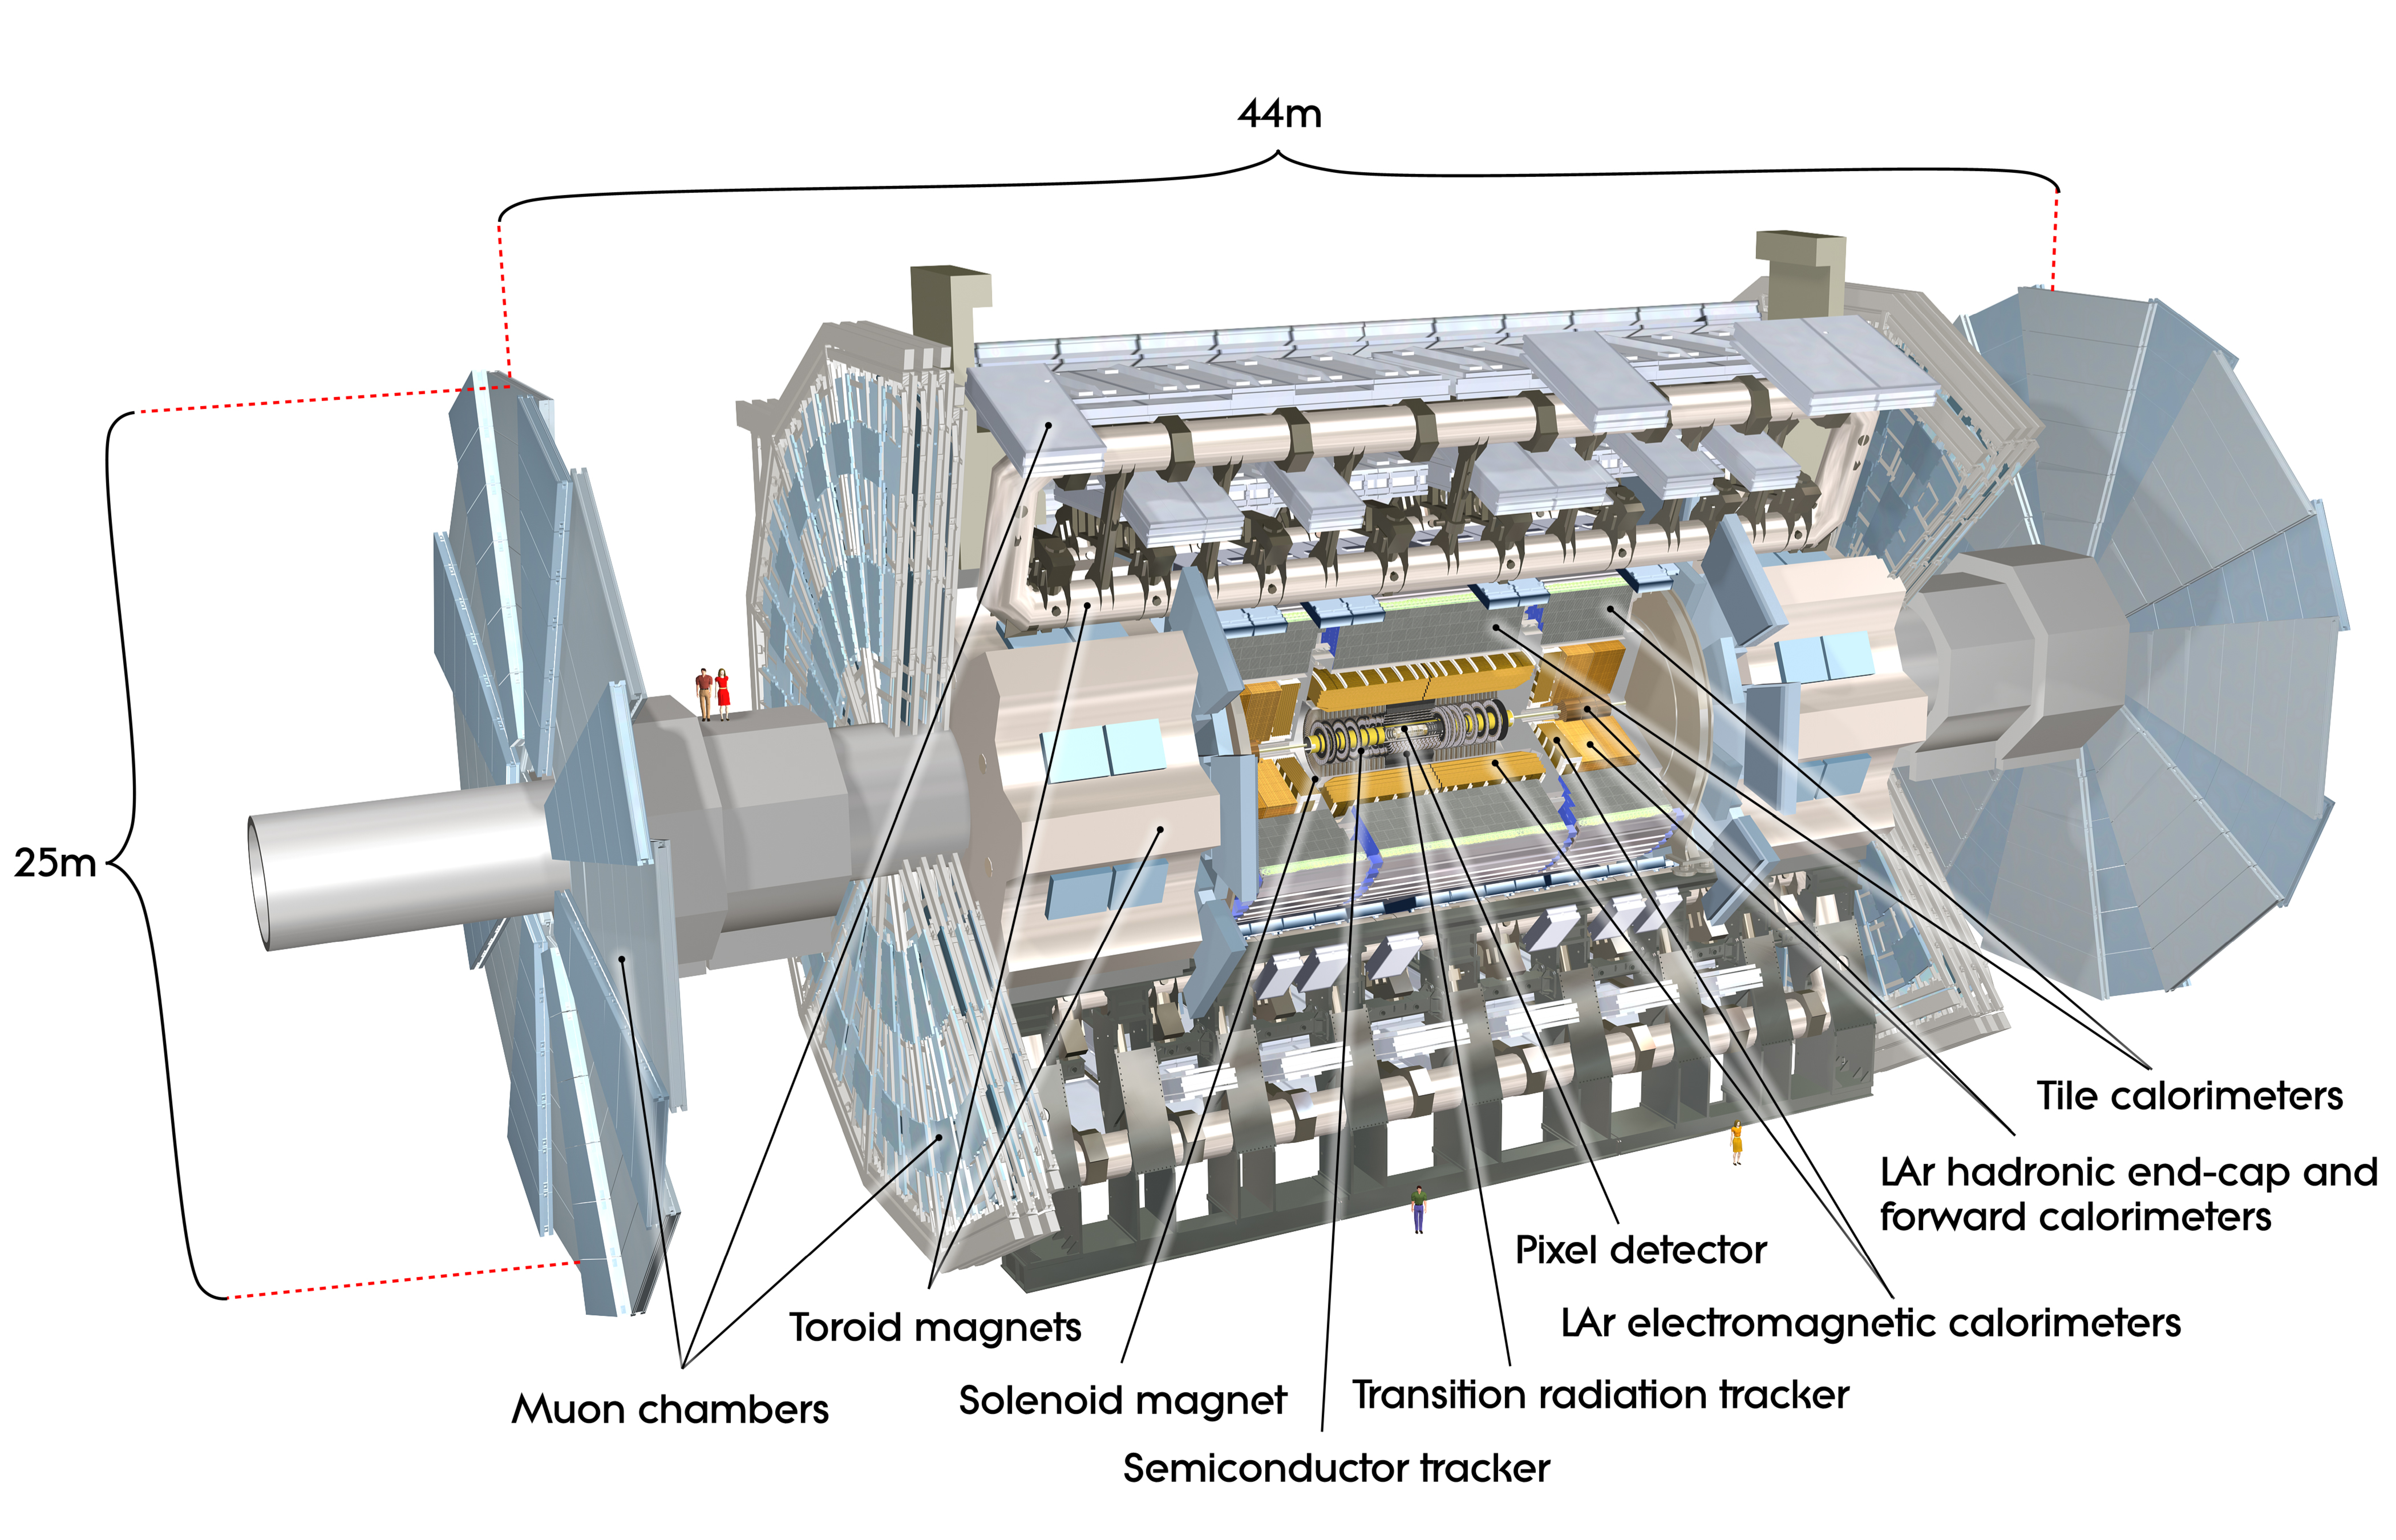
\includegraphics[width=125mm]{ATLAS_Detector_overview}

    \includegraphics[width=100mm]{ATLAS_ID}
  \end{center}
  \caption{An overview diagram of the ATLAS detector (top) and a diagram of the Inner Detector tracking systems (bottom).}
  \label{fig:ATLAS_overview}
\end{figure}

%\cite{CERN:images_overview}
%\cite{CERN:images_id}
\subsection{Inner Detector}

The Inner Detector (ID) is primarily a silicon based tracking system designed to reconstruct charged particle tracks down to a tranverse momentum ($p_{T}$) of $~0.5\, GeV$. It covers the full $\phi$ angle and provides tracking up to $|\eta|< 2.5$. It also provides some rudimentary particle identification via transition radiation.
 
%\subsubsubsection{Pixel Detector}
The Pixel Detector is the central most detector in ATLAS, situated just 50.5 mm away from the beam line in the inner most layer. It consists of three layers of silicon pixel modules in the central barrel, and five disk layers in the high $\eta$ end cap regions. The detector contains 1744 sensors, each with 47232 pixes with dimensions $50 \times 400~\mu m^2$. The detector is exposed to intense radiation and as such must be exteremely radiation hard to allow precision tracking measurements. During the first upgrade, the current pixel detector with be augmented with an additional layer, the insertable b-layer (IBL), to provide improved accuracy and vertex identification. 

%\subsubsubsection*{Semi Condictor Tracker (SCT)}
Continuing outwards from the Pixel Detector one encoutners the SCT. While also a silicon based technology, the SCT is a strip based detector rather than a pixel detector. Twi strips are places at small stero angles in 4 layers to allow for 4 individual space point measurements (in a total of 8 layers). The small stero angle (16 micro radians?) reduces the number of ambiguous space point solutions. When combined with the global position of the modules, a 3D space point can be constructed just as in the pixel detector, though the technology is cheaper and easier to scale to the large surface areas required by the SCT.

%\subsubsubsection*{Transition Radiation Tracker (TRT)}
The final part of the inner detector is the transition radiation tracker (TRT). Unlike the other two silicon based layers, this layer is designed from straw tube technology.

\subsection{The Calorimeter}
%\subsubsubsection*{Electron Magnetic Calorimeter (EMCalo)}
%\subsubsubsection*{Hadronic Calorimeter (HCal)}
%\subsubsubsection*{Forward Calorimeters}

\subsection{Magnet Systems}
%\subsubsubsection*{Solenoid}
%\subsubsubsection*{Toroid}

\subsection{Muon Systems}
%\subsubsubsection*{Monitored Drift Tubes (MDTs)}
%\subsubsubsection*{Resistive Plate Chambers (RPCs)}
%\subsubsubsection*{Cathode Strip Chambers (CSCs)}
%\subsubsubsection*{Thin Gap Chambers (TGCs)}

\subsection{Other detectors}
%\subsubsubsection*{Minium Bias Scintilator Tiles (MBTS)}
%\subsubsubsection*{Beam Conditions Monitor (BCM)}

\section{ATLAS Trigger System}
\subsection{Level 1, Level 2 and Event Filter}

\section{Object Identification and Reconstruction}

\subsection{Electrons}
\label{sec:electrons}
 Electrons are reconstucted in ATLAS by combining EM calorimeter showers with inner detector tracks. Due to the limitations in the tracker, electrons are only reconstructed at $\eta < 2.47$ with the crack regions excluded ($1.37 < |\eta_{cluster}| < 1.52$). Electrons are required to have a $E_{T(corrected)} > 25 \GeV~$ where $E_{T(corrected)} = E_{cluster} / cosh(\eta_{track})$. In addition strict cuts are placed on the calorimeter shower shapes to require a central energy maximum to distinguish electrons from other jet signatures. 

\subsection{Muons}
\label{sec:muons}
Muons in ATLAS are reconstructed using the 'muid' algorithm that matches inner detector tracks with tracks in the Muon spectrometer. These types of muons are so called 'combined' muons. Due to detector acceptence limitations muons may only be reconstructed with $\eta < 2.5$. In order to ensure that muons are selected in a stable plateau of trigger efficiency at \pt~ cut of greater than 20 \GeV~ is imposed. Backgrounds of prompt muons are dominated by heavy flavour decays. In order to supress these a combination of isolation cuts are used. The sum \pt~ of tracks inside a delta R cone of 0.3 must be less than 2.5 GeV and the sum \et~ of must be less than 4 \GeV~ in the same cone size\cite{ATLAS:Top_dilep_xsec}. The values for these isolation cuts were optimised to provide high efficiency regardless of pileup. Finally, muons that overlap with a selected jet within a delta R of 0.4 are rejected. 

Muons are triggered using two algorithms; mu18 and mu18medium. For earlier data periods with low pileup mu18 is used. This is changed to the medium algorithm in later periods in order to maintain the trigger unprescaled at high efficiency in the presence of high pileup.

(find plot of reco efficiency and trigger efficiency)

\subsection{Jets}
\label{sec:jets}
Try to summarise Jets at ATLAS in a way that doesn't become a thesis by itself! Algorithm used: anti $K_{T}$ with cone size of 0.4 (also 0.6 for some QCD studies). EM Scale calibrated, pileup supression using inner detector tracks. 

\subsection{Missing Energy}
\label{sec:met}
Put up the huge formula for the \etmiss and all of its components. Show the study of \etmiss resolution as a function of sumET. 

\subsection{Photons, Pions and other signatures}
Briefly mention about pion reconstruction (mainly for Tau signatures?), Photons (since they're the natural converse to Electrons) and any other signatures that you can think of.






